% LaTeX Article Template
\documentclass[12pt]{article}
%% Other packages
\usepackage{amsmath}
\usepackage{amsthm}
\usepackage{titlesec}
\usepackage{soul}
\usepackage{tikz}
\usepackage{tikz-3dplot}
\usepackage{amssymb}
\usepackage{multicol}
\usepackage{float}
\usepackage{calc}
\usepackage{fancybox}
\usepackage{array}
\usepackage[shortlabels]{enumitem}
\usepackage{framed}
\usepackage{hyperref}
\newcolumntype{L}[1]{>{\raggedright\let\newline\\\arraybackslash\hspace{0pt}}m{#1}}
\newcolumntype{C}[1]{>{\centering\let\newline\\\arraybackslash\hspace{0pt}}m{#1}}
\newcolumntype{R}[1]{>{\raggedleft\let\newline\\\arraybackslash\hspace{0pt}}m{#1}}


%% Margins
\usepackage{geometry}
\geometry{verbose,letterpaper,tmargin=1in,bmargin=1in,lmargin=1in,rmargin=1in}

\newcommand{\menuchoice}[2]{{\ttfamily#1..#2}}
\newcommand{\dotdot}{..}

\usepackage{graphicx}

% Array vertical and horizontal stretch
% \def\arraystretch{1.5}%  1 is the default, change whatever you need
% \setlength{\tabcolsep}{12pt}

%\graphicspath{%
\graphicspath{{./figs/}}

%% Paragraph style settings
\setlength{\parskip}{\medskipamount}
\setlength{\parindent}{0pt}

%% Change itemize bullets
\renewcommand{\labelitemi}{$\bullet$}
\renewcommand{\labelitemii}{$\circ$}
\renewcommand{\labelitemiii}{$\diamond$}
\renewcommand{\labelitemiv}{$\cdot$}

%% Shrink section fonts
\titleformat*{\section}{\large\bf}
\titleformat*{\subsection}{\normalsize\it}
\titleformat*{\subsubsection}{\normalsize\bf}

% %% Compress the spacing around section titles
\titlespacing*{\section}{0pt}{1.5ex}{0.75ex}
\titlespacing*{\subsection}{0pt}{1ex}{0.5ex}
\titlespacing*{\subsubsection}{0pt}{1ex}{0.5ex}

%% amsthm settings
\theoremstyle{definition}
\newtheorem{problem}{Problem}
\newtheorem{example}{Example}
\newtheorem{mydef}{Definition}

%% Answer box macros
%% \answerbox{alignment}{width}{height}
\newcommand{\answerbox}[3]{%
  \fbox{%
    \begin{minipage}[#1]{#2}
      \hfill\vspace{#3}
    \end{minipage}
  }
}

%% \answerboxfull{alignment}{height}
\newcommand{\answerboxfull}[2]{%
  \answerbox{#1}{\textwidth}{#2} 
}

%% \answerboxone{alignment}{height} -- for first-level bullet
\newcommand{\answerboxone}[2]{%
  \answerbox{#1}{6.15in}{#2} 
}

%% \answerboxtwo{alignment}{height} -- for second-level bullet
\newcommand{\answerboxtwo}[2]{%
  \answerbox{#1}{5.8in}{#2}
}

%% \graphbox{xmin}{xmax}{ymin}{ymax}{scale}
\newcommand{\graphbox}[5]%[-5, 5, -5, 5, 0.33]
{
\begin{tikzpicture}
     [>=latex,scale=#5]
     
     % Coordinate axes
     \draw [->,very thick] (#1, 0) -- (#2, 0) node[right] {$x$};
     \draw [->,very thick] (0, #3) -- (0, #4) node[above] {$y$};
     
     % Grid
     \draw[step=1cm,thick,dotted] (#1,#3) grid (#2,#4);
   \end{tikzpicture}
   }


%% Redefine maketitle
\makeatletter
\renewcommand{\maketitle}{
  \noindent SA403 -- Networks \\

  \begin{center}\Large{\textbf{\@title}}\end{center}
}
\makeatother

% Set the beginning of a LaTeX document
\begin{document}

%\graphbox{-10}{3}{-5}{10}

\title{Lesson 5: Minimum Spanning Tree}

%\graphbox[10][10]

\maketitle


\section*{Notes}

Book acknowledgment:
\section*{Goals}
\begin{itemize}
\item Minimum Spanning Tree
\end{itemize}


\section{Try it on your own}

For the network below, determine the minimum cumulative weight spanning tree.

\begin{center}
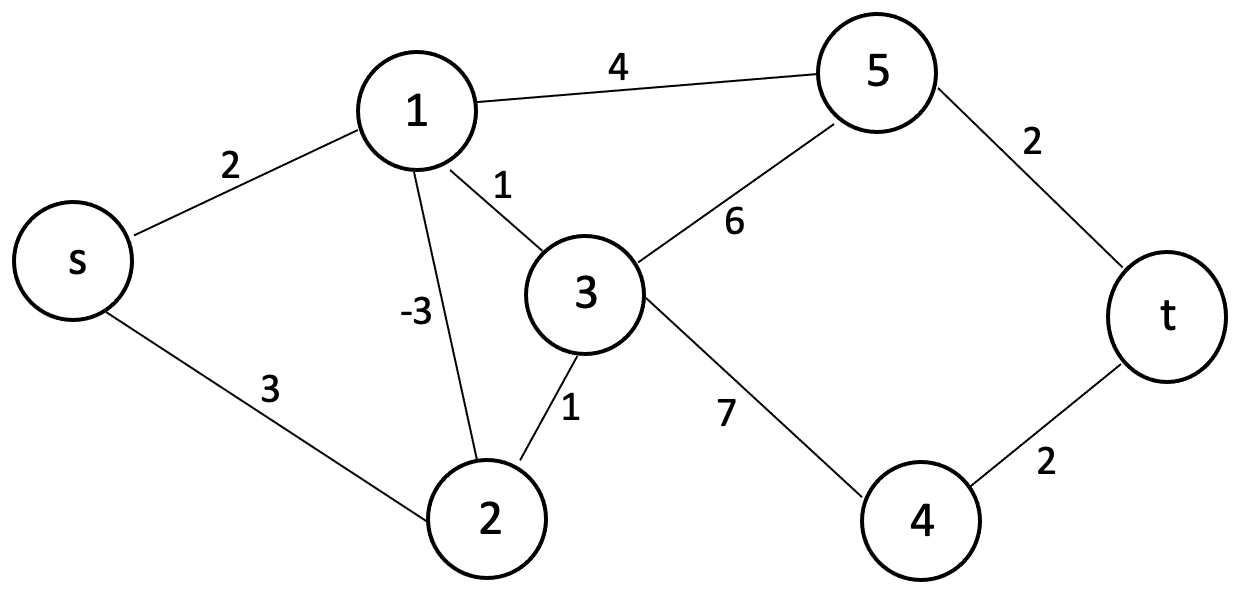
\includegraphics[width=10cm]{minspanningtree}
\end{center}

\vfill

What is your solution? How did you determine it? Can you transform your strategy into an algorithm?\vfill
\newpage
\section{Problem Definition}

Given a graph $G = (V,E)$, in which edge $(i,j) \in E$ has a weight $w_{ij}$. Determine the subset of edges of a connected subgraph that connects all the vertices without any cycles and with the minimum cumulative edge weights. In other words, determine a spanning tree whose cumulative edge weights is as small as possible.

How many edges will a minimum spanning tree have?


\vfill

Given your current knowledge, how would you go about solving this problem?
\vfill

\newpage
\section{Kruskal's Algorithm}

Kruskal's Algorithm is a greedy algorithm that chooses the smallest weight edge to include in the MST that does not create a cycle in the current MST.

\textbf{Steps:}

\begin{enumerate}
	\item Sort all the edges in $E$ in non-decreasing order of their weight. Set $T = \emptyset$.
	\item While $|T| < |V|$:
	\begin{enumerate}
		\item Pick the smallest weight edge $(i,j)$. If edge $(i,j)$ doest not form a cycle among the edges in $T$, then add $(i,j)$ to $T$. Remove $(i,j) in E$. 
	\end{enumerate}
\end{enumerate}

\vfill

How would you go about sorting the edges in $E$ according to their weight? 

\vfill

How would you check to see if adding $(i,j)$ to $T$ would create a cycle?
\vfill

\newpage

For the network below, determine the MST using Kruskal's Algorithm.

\begin{center}
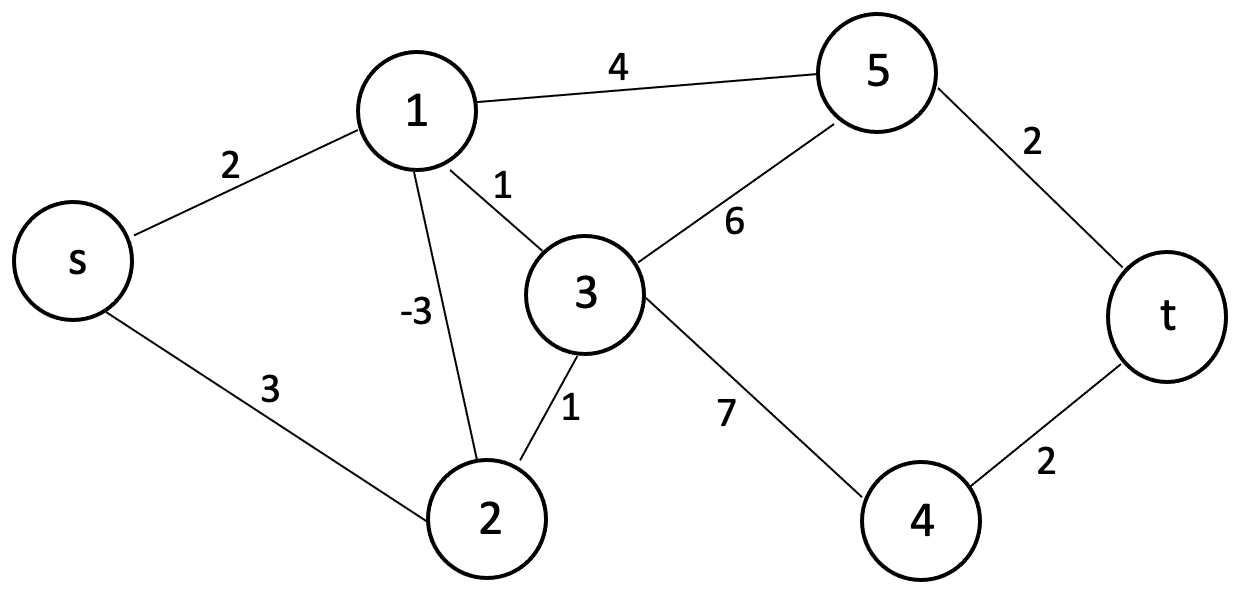
\includegraphics[width=10cm]{minspanningtree}
\end{center}


\newpage
\section{Prim's Algorithm}

Like Kruskal's Algorithm, Prim's Algorithm is a greedy approach. It starts with an empty spanning tree that maintains two sets of nodes. The former set contains the nodes included in the MST, and the latter set contains the nodes not yet included in the MST. At each step, Prim's considers all the edges that connect the two sets, and picks the minimum weight edges from among these edges. After picking the edge, Prim's moves one node from the latter set to the former set. The group of edges that connects the two sets is referred to as a \emph{cut}. 

\textbf{Steps:}

\begin{enumerate}

	\item Initialize $T = \emptyset$.
	\item Set $v_i = \infty, \ \forall i \in V$, and set $v_s = 0$.
	\item While $|T| < |V|$:
	\begin{enumerate}
		\item Pick a node $u \in V \setminus T$ for which $v_u = \textrm{min}\{v_i: i \in V \setminus T \}$.
		\item Add $u$ to $T$.
		\item Update $v_i$ for each node $i$ adjacent to $u$. For all $(u,i) \in E$, if $v_i > c_{ui}$, then set $v_i = v_u + c_{ui}$.
	\end{enumerate}
For the network below, determine the MST using Prim's Algorithm.

\begin{center}
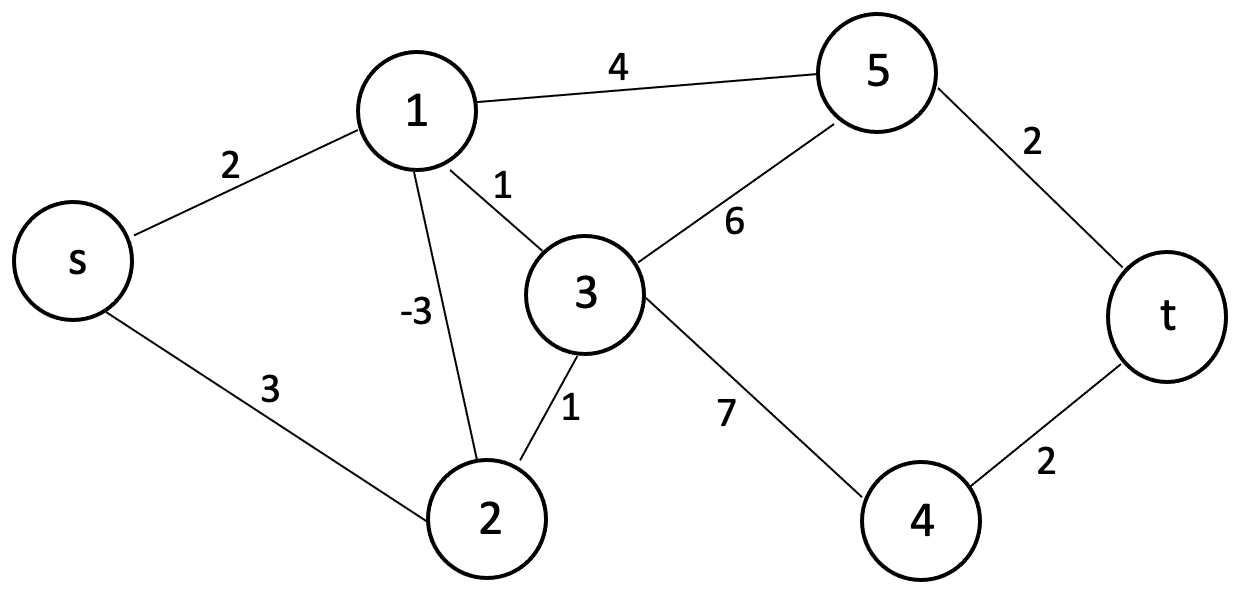
\includegraphics[width=10cm]{minspanningtree}
\end{center}


\newpage

\end{enumerate}


\section{Kruskal's vs. Prim's}

\begin{itemize}
	\item Kruskal's Algorithm tends to run faster in sparse graph, while Prim's Algorithm tends to run faster in dense graphs.
	\item Prim's starts to build the MST from any node in the graph, while Kruskal's builds a MST from the vertex carruying minimum weight in the graph.
	\item Kruskal's Algorithm traverses one node only once, while Prim's Algorithm traverse one node more than once time to the get the minimum distance.
	\item Prim's Algorithm gives connected components and works only on connected graphs, while Kruskal's Algorithm can generate disconnected components.
	\item Prim's Algorithm runs in $O(V^2)$ time, and Kruskal's Algorithm runs in $O(E \ \textrm{log}(V))$ time.
\end{itemize}


\end{document}
